\chapter*{บทที่ 3 การออกแบบระบบ}\addcontentsline{toc}{chapter}{บทที่ 3 การออกแบบระบบ}

\section*{3.1 สถาปัตยกรรมระบบ}\addcontentsline{toc}{section}{3.1 สถาปัตยกรรมระบบ}

ระบบทั้งหมดทำงานบนเซิร์ฟเวอร์เสมือนเครื่องเดียว ทุกการเชื่อมต่อขาเข้าต้องผ่าน geo-firewall ก่อนถึงบริการใดๆ และฐานข้อมูลรับการเชื่อมต่อเฉพาะจากภายในเครื่อง

\begin{center}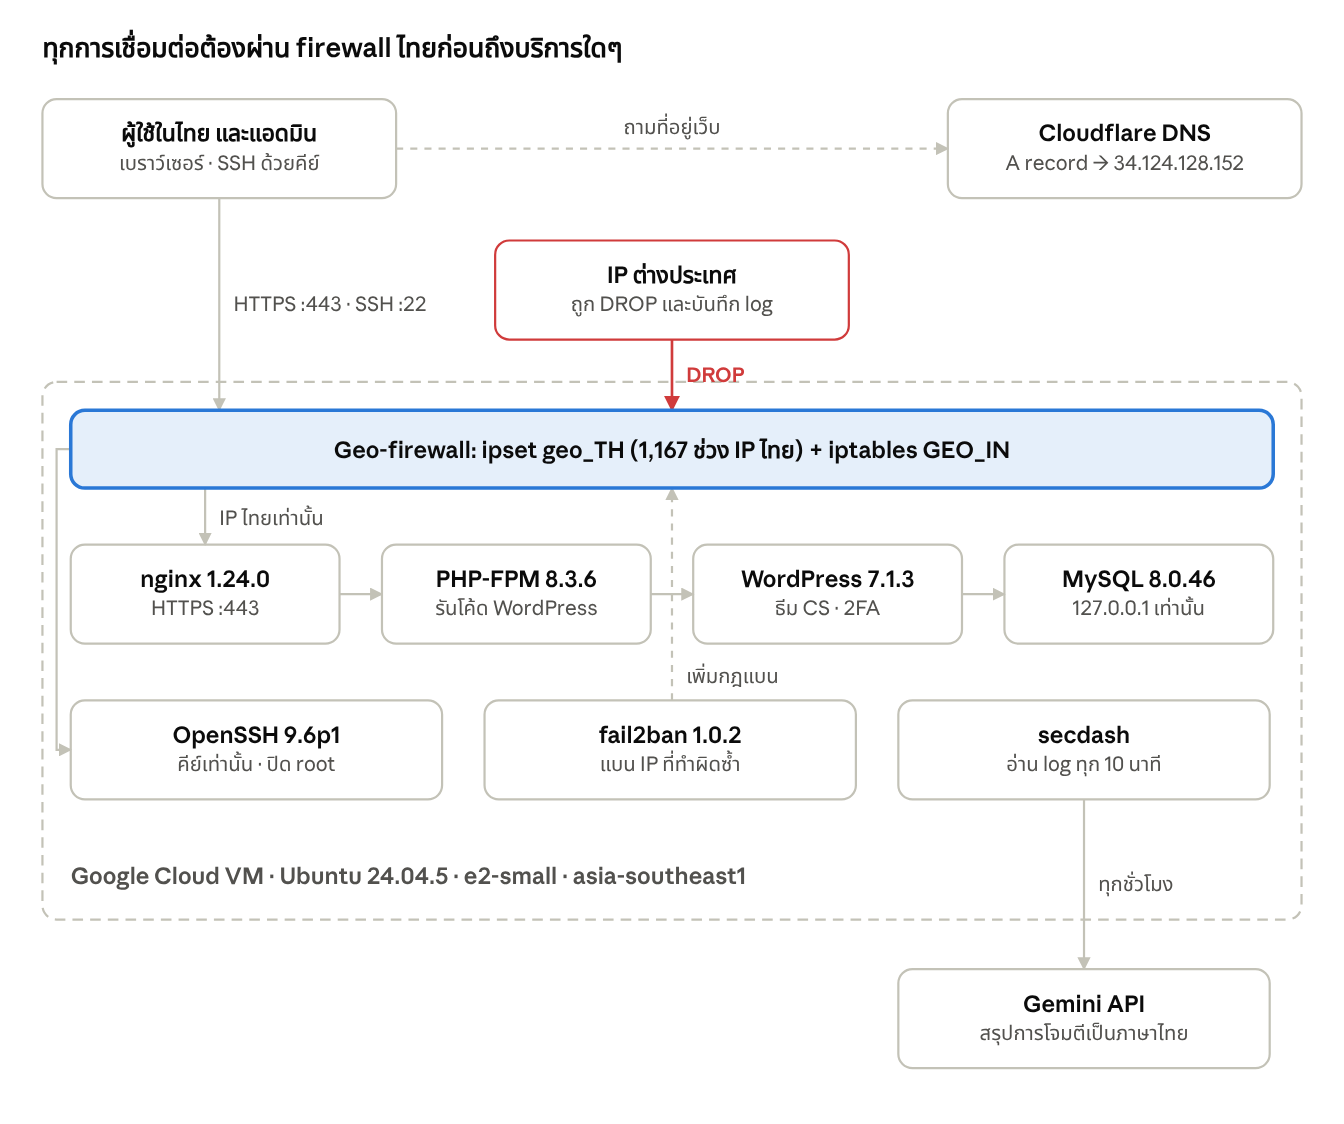
\includegraphics[width=0.95\linewidth,keepaspectratio]{figures/architecture.png}\end{center}

ภาพที่ 3.1 ผู้ใช้ถาม DNS แล้วเชื่อมต่อเซิร์ฟเวอร์ ทุกการเชื่อมต่อผ่าน geo-firewall ก่อน IP ไทยไปถึง nginx หรือ OpenSSH ส่วน IP ต่างประเทศถูก DROP และ secdash อ่าน log ทุกส่วนแล้วส่งสรุปให้ Gemini ทุกชั่วโมง

ตารางที่ 3.1 ซอฟต์แวร์และเวอร์ชันที่ใช้ (จากไฟล์ versions.txt บนเซิร์ฟเวอร์)

\begin{longtable}[]{@{}>{\raggedright\arraybackslash}p{0.282\linewidth - 2\tabcolsep}>{\raggedright\arraybackslash}p{0.395\linewidth - 2\tabcolsep}>{\raggedright\arraybackslash}p{0.293\linewidth - 2\tabcolsep}@{}}
\toprule\noalign{}
ส่วนประกอบ & เวอร์ชัน & หน้าที่ \\
\midrule\noalign{}
\endhead
\bottomrule\noalign{}
\endlastfoot
Ubuntu Server & 24.04.5 LTS (kernel 7.0.0-1014-gcp) & ระบบปฏิบัติการ \\
nginx & 1.24.0 & เว็บเซิร์ฟเวอร์ และ HTTPS \\
PHP-FPM & 8.3.6 & รันโค้ด WordPress \\
MySQL & 8.0.46 & ฐานข้อมูล \\
WordPress & 7.1.3 & ระบบจัดการเนื้อหา \\
OpenSSH & 9.6p1 & เข้าเซิร์ฟเวอร์ด้วยกุญแจ \\
fail2ban & 1.0.2 & แบน IP ที่ทำผิดซ้ำ \\
acme.sh & ใบรับรองจาก Let's Encrypt & ออกและต่ออายุใบรับรอง \\
ipset + iptables & ตามที่ Ubuntu ให้มา & geo-firewall \\
Python 3 (ไลบรารีมาตรฐาน) & ตามที่ Ubuntu ให้มา & ตัวเก็บข้อมูล secdash \\
\end{longtable}

คณะผู้จัดทำซ่อนเวอร์ชันเหล่านี้จากภายนอก (server\_tokens off และ expose\_php Off) เพื่อไม่ให้ผู้โจมตีเลือกช่องโหว่ที่ตรงกับเวอร์ชันได้ง่าย

\section*{3.2 การไหลของคำขอ}\addcontentsline{toc}{section}{3.2 การไหลของคำขอ}

\begin{enumerate}
\def\labelenumi{\arabic{enumi}.}
\tightlist
\item
  ผู้ใช้พิมพ์ elephotelephus.site เบราว์เซอร์ถาม DNS ของ Cloudflare และได้ IP 34.124.128.152
\item
  เบราว์เซอร์เชื่อมต่อพอร์ต 443 การเชื่อมต่อผ่าน firewall ของ Google Cloud แล้วเข้าสู่ chain GEO\_IN ของ iptables
\item
  ถ้า IP ต้นทางอยู่ในชุด IP ไทย แพ็กเก็ตผ่านไปถึง nginx ถ้าไม่ใช่ จะถูกบันทึก log และ DROP
\item
  nginx ถอดรหัส TLS ตรวจกฎความปลอดภัย (เช่น ปฏิเสธ xmlrpc.php และไฟล์ที่ขึ้นต้นด้วยจุด) แล้วส่งคำขอ PHP ให้ PHP-FPM
\item
  WordPress อ่านข้อมูลจาก MySQL ผ่าน 127.0.0.1 สร้างหน้าเว็บ และส่งกลับผ่าน nginx
\end{enumerate}

ผู้ดูแลระบบเข้าเครื่องด้วย SSH ผ่านพอร์ต 22 ซึ่งต้องผ่าน geo-firewall เช่นกัน ส่วนการดูฐานข้อมูลจากเครื่องของตนเอง (เช่น ด้วย DBeaver) ทำผ่าน SSH tunnel โดยไม่เปิดพอร์ต 3306 สู่อินเทอร์เน็ต

\section*{3.3 การป้องกันหลายชั้น (Defense in depth)}\addcontentsline{toc}{section}{3.3 การป้องกันหลายชั้น (Defense in depth)}

คณะผู้จัดทำไม่พึ่งการป้องกันชั้นเดียว เพราะผู้โจมตีอาจใช้ IP ไทย เช่น VPN หรือเครื่องในไทยที่ถูกยึด แต่ละชั้นจึงรับมือการโจมตีคนละแบบ

ตารางที่ 3.2 มาตรการป้องกันแต่ละชั้น

\begin{longtable}[]{@{}>{\raggedright\arraybackslash}p{0.115\linewidth - 2\tabcolsep}>{\raggedright\arraybackslash}p{0.427\linewidth - 2\tabcolsep}>{\raggedright\arraybackslash}p{0.427\linewidth - 2\tabcolsep}@{}}
\toprule\noalign{}
ชั้น & มาตรการ & รับมือกับ \\
\midrule\noalign{}
\endhead
\bottomrule\noalign{}
\endlastfoot
เครือข่าย & Geo-firewall รับเฉพาะ IP ไทย · fail2ban & บอทสแกนจากต่างประเทศ · การเดารหัสซ้ำ \\
การเข้าเครื่อง & SSH กุญแจเท่านั้น · ปิด root · บัญชีแยกรายบุคคล & การเดารหัส SSH · การยึดสิทธิ์ root \\
เว็บเซิร์ฟเวอร์ & ซ่อนเวอร์ชัน · security headers · จำกัดความถี่ wp-login (429) · ปิด xmlrpc.php · ปฏิเสธไฟล์ .env/.git · ห้ามรัน PHP ในโฟลเดอร์ uploads & การสำรวจระบบ · brute force · การสแกนไฟล์ลับ · การอัปโหลด web shell \\
WordPress & 2FA · ชื่อผู้ดูแลเดายาก · DISALLOW\_FILE\_EDIT · ลบธีม/ปลั๊กอินที่ไม่ใช้ · escape ข้อความทุกส่วน & รหัสผ่านรั่ว · การแก้โค้ดผ่านหลังบ้าน · XSS \\
ฐานข้อมูล & MySQL รับเฉพาะ 127.0.0.1 · ผู้ใช้ DB เฉพาะของ WordPress · เข้าดูผ่าน SSH tunnel & การเชื่อมต่อฐานข้อมูลจากภายนอก \\
ดูแลระบบ & unattended-upgrades · สำรองข้อมูลทุกวัน · swap & ช่องโหว่ที่มีแพตช์แล้ว · ข้อมูลเสียหาย \\
เฝ้าระวัง & secdash + AI (บทที่ 5) & มองเห็นการโจมตีที่เกิดขึ้นจริง \\
\end{longtable}
